%================================================================
% 作業ログ テンプレート
%   教員配布の「作業ログ_配布.pdf」と同じ章構成・要素・階層を LaTeX で再現。
%   実際の作業ログを書くときは本ファイルをコピーして書き換える。
%
%   ビルド:
%     cd report/作業ログテンプレート
%     docker run --rm -v "$(pwd):/workspace" -w /workspace \
%       ghcr.io/paperist/texlive-ja:debian latexmk 作業ログテンプレート.tex
%   出力: 作業ログテンプレート.pdf（配布原本とは別ファイル）
%================================================================
\documentclass[uplatex,dvipdfmx,a4paper,11pt]{jsarticle}

% --- 余白 ---
\usepackage[top=25mm,bottom=25mm,left=25mm,right=25mm]{geometry}

% --- 表・箇条書き・図 ---
\usepackage{array}
\usepackage{tabularx}
\usepackage{booktabs}
\usepackage{enumitem}
\usepackage{graphicx}

% --- 段落間隔（Wordのような見た目に寄せる）---
\setlength{\parindent}{0pt}
\setlength{\parskip}{0.6em}

% --- セクション見出しを「番号. 太字」+ 章末に水平線を入れる ---
\usepackage{titlesec}
\titleformat{\section}
  {\normalfont\Large\bfseries}{\thesection.}{0.6em}{}
\titleformat{\subsection}
  {\normalfont\large\bfseries}{\thesubsection}{0.6em}{}
\titlespacing*{\section}{0pt}{1.2em}{0.6em}
\titlespacing*{\subsection}{0pt}{1.0em}{0.4em}

% --- 章末水平線（手で \sectionrule と書いて区切る）---
\newcommand{\sectionrule}{\par\medskip\noindent\rule{\linewidth}{0.6pt}\par\medskip}

% --- 箇条書きの記号を Word 風（・→○→数字）に揃える ---
\renewcommand{\labelitemi}{\textbullet}
\renewcommand{\labelitemii}{\textopenbullet}
\setlist[itemize]{leftmargin=1.6em,itemsep=0.1em,topsep=0.2em}
\setlist[enumerate]{leftmargin=2.0em,itemsep=0.1em,topsep=0.2em}

% \textopenbullet が無い環境向けのフォールバック（jsarticle標準では○が出る）
\providecommand{\textopenbullet}{\ensuremath{\circ}}

\begin{document}

%================================================================
% ヘッダ
%================================================================
{\LARGE\bfseries 作業ログ}\par\bigskip

報告者：齋藤　翔太

報告日：2026年5月27日

プロジェクト名：タクトーン〜IMUジェスチャーで奏でるArduinoオーケストラ〜

\sectionrule

%================================================================
% 1. 進捗サマリー
%================================================================
\section{進捗サマリー（要約）}

\begin{itemize}
  \item 全体進捗率：60％
  \item マイルストーン達成状況：予定通り進行中
  \item 主要成果：
    \begin{itemize}
      \item {}担当タスクである「4パート楽譜のヘッダ配列化」に向けて，
        課題曲を「きらきら星」とし，金管4パートを0／4／8／12拍
        ずらして演奏する輪唱構成を整理した．
      \item {}Arduinoへ楽譜を組み込む前に音階と発音タイミングを確認するため，
        固定テンポで金管4パートを再生できるProcessingデバッグ用
        スケッチを作成した．
      \item {}結合後計画書の楽譜データ形式に合わせ，
        細分音符用の\texttt{subNote}等を含む\texttt{ScoreEvent}形式で，
        Arduino統合用の楽譜データを作成した．
    \end{itemize}
  \item 重大課題（影響度：高）：
    \begin{itemize}
      \item {}作成した4声輪唱は，現時点では実音による確認を行っていない．
        次回作業でProcessing上の試聴確認を行い，必要に応じて楽譜データを修正する．
    \end{itemize}
\end{itemize}

\sectionrule

%================================================================
% 2. 作業ログ（詳細トラッキング）
%================================================================
\section{作業ログ（詳細トラッキング）}

{\footnotesize
\renewcommand{\arraystretch}{1.25}
\begin{tabularx}{\linewidth}{@{}>{\raggedright\arraybackslash}p{21mm}>{\raggedright\arraybackslash}p{13mm}>{\raggedright\arraybackslash}p{17mm}>{\raggedright\arraybackslash}p{16mm}>{\raggedright\arraybackslash}p{12mm}XX@{}}
\toprule
作業項目 & 開始日 & 予定完了日 & 状態 & 進捗率 & 依存関係・ブロッカー & コメント \\
\midrule
課題曲と輪唱構成の整理
  & 5/13 & 5/13 & 完了 & 100\%
  & なし
  & 「きらきら星」を金管4声で演奏する構成を整理した． \\
Processing確認用スケッチの作成・試聴
  & 5/24 & 5/31 & 進行中 & 80\%
  & Minimの導入，実音確認
  & 4声を再生するスケッチは作成済みであり，試聴が残っている． \\
Arduino統合用楽譜データの作成
  & 5/25 & 5/31 & レビュー中 & 70\%
  & ファームウェアへの統合
  & 48拍分の\texttt{ScoreEvent}データとパート設定を作成した． \\
ファームウェア反映・ROM埋込確認
  & 未着手 & 6/2 & 未着手 & 0\%
  & 塩澤担当実装との統合
  & \texttt{firmware/}への反映および実機確認は未実施である． \\
\bottomrule
\end{tabularx}
}

\newpage
\subsection{日ごとの作業時間・作業内容}

{\footnotesize
\renewcommand{\arraystretch}{1.25}
\begin{tabularx}{\linewidth}{@{}>{\raggedright\arraybackslash}p{16mm}>{\raggedright\arraybackslash}p{22mm}XX@{}}
\toprule
日付 & 作業時間 & 作業内容 & 成果・残課題 \\
\midrule
5/13
  & \textbf{1.5}時間
  & 課題曲と輪唱構成の整理
  & 「きらきら星」を金管4声で演奏する構成を整理した． \\
5/24
  & \textbf{4}時間
  & Processing確認用スケッチの作成
  & 4声を再生するスケッチを作成した．実音による試聴確認が残っている． \\
5/25
  & \textbf{4}時間
  & Arduino統合用楽譜データの作成
  & 48拍分の\texttt{ScoreEvent}データとパート設定を作成した． \\
5/26
  & \textbf{5}時間
  & 作成物の再確認と作業ログの整理
  & 作成物の整合性を確認し，作業ログを整理した． \\
\bottomrule
\end{tabularx}
}

\sectionrule

%================================================================
% 3. 担当箇所の計画前GCと現在のGC
%================================================================
\section{担当箇所の計画前GCと現在のGC}

担当箇所について，計画前に設定したGCから現時点で予定日程の変更はない．
したがって，計画前のGCと現在のGCは同一であり，図\ref{fig:saito-gc}に
両者共通のGCを示す．

\begin{figure}[htbp]
  \centering
  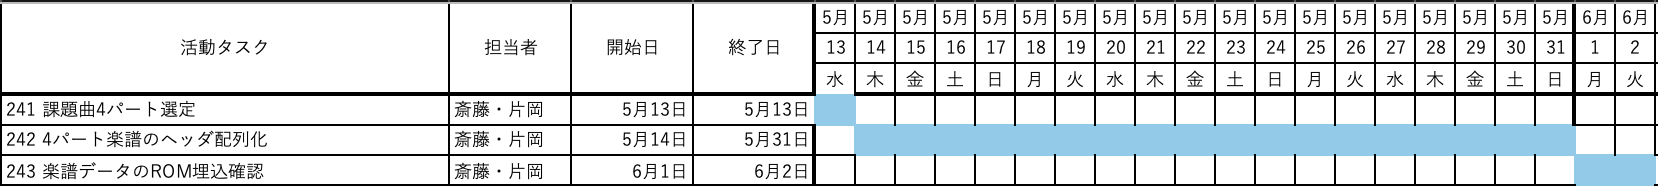
\includegraphics[width=\linewidth]{Figs/my_GC.png}
  \caption{担当箇所のGC（計画前・現在共通）}
  \label{fig:saito-gc}
\end{figure}

\sectionrule

%================================================================
% 4. 課題管理
%================================================================
\section{課題管理}

{\footnotesize
\renewcommand{\arraystretch}{1.25}
\begin{tabularx}{\linewidth}{@{}>{\raggedright\arraybackslash}p{25mm}X>{\raggedright\arraybackslash}p{11mm}>{\raggedright\arraybackslash}p{11mm}X>{\raggedright\arraybackslash}p{19mm}>{\raggedright\arraybackslash}p{17mm}@{}}
\toprule
課題 & 発生原因 & 影響度 & 優先度 & 対策 & 期限 & 状態 \\
\midrule
4声輪唱の実音未確認
  & 確認用スケッチの作成後，試聴結果をまだ記録していない．
  & 中 & 高
  & Processingで再生し，音の重なりを確認する．
  & 次回作業時 & 未対応 \\
ROM埋込確認の未実施
  & 楽譜データがファームウェアへ未統合である．
  & 中 & 中
  & ファームウェアへの統合後にビルドおよび実機確認を行う．
  & 統合後 & 未対応 \\
\bottomrule
\end{tabularx}
}

\sectionrule

%================================================================
% 5. AI利用状況と検証
%================================================================
\section{AI利用状況と検証（再現性重視）}

\subsection{利用内容}

\begin{itemize}
  \item 利用目的：作業ログの記載項目確認，文章表現の整理
  \item 入力（プロンプト要旨）：
    \begin{itemize}
      \item {}提出要件に対して記入漏れがないかを確認し，記載内容を整理するよう依頼した．
    \end{itemize}
  \item 出力概要：
    \begin{itemize}
      \item {}GC，日ごとの作業時間・作業内容，次回実施内容の記載を整理した．
    \end{itemize}
\end{itemize}

\sectionrule

\subsection{検証方法}

\begin{itemize}
  \item 検証手法：
    \begin{itemize}
      \item {}提出要件とリポジトリに存在する成果物を確認し，
        作業ログの記載内容と照合した．
    \end{itemize}
  \item 参照資料：
    \begin{itemize}
      \item {}\texttt{work/saito/week5/arduino\_score\_draft/}内の楽譜データ
      \item {}\texttt{work/saito/week5/kirakira\_score\_debug/}内の試聴用スケッチ
      \item {}\texttt{meetings/0422\_2回/wbs\_table/wbs\_table.md}
    \end{itemize}
  \item 検証手順：
    \begin{enumerate}
      \item {}楽譜データとProcessingスケッチの存在および内容を確認した．
      \item {}WBSに記載された齋藤担当タスクと，作成済み成果物を対応付けた．
      \item {}日ごとの作業内容，GC，次回実施内容が記載されていることを確認した．
    \end{enumerate}
\end{itemize}

\sectionrule

\subsection{ファクトチェック結果}

\begin{itemize}
  \item 一致点：
    \begin{itemize}
      \item {}\texttt{ScoreEvent}形式の48拍分楽譜データと，
        Processing確認用スケッチが作成されていることを確認した．
    \end{itemize}
  \item 不一致・疑義：
    \begin{itemize}
      \item {}試聴確認およびROM埋込確認は未実施であり，次回作業で確認する必要がある．
    \end{itemize}
  \item 最終判断：
    \begin{itemize}
      \item 作成済み成果物は今回の進捗として記載し，
        未実施の確認作業は次回実施内容として記載する．
    \end{itemize}
  \item 根拠：
    \begin{itemize}
      \item {}楽譜データ・試聴用スケッチの実ファイルと，
        WBSおよび提出要件を照合した結果による．
    \end{itemize}
\end{itemize}

\sectionrule

%================================================================
% 6. 次回計画
%================================================================
\section{次回計画}

\begin{itemize}
  \item 目標：
    \begin{itemize}
      \item {}Processingスケッチを用いて音の重なりを試聴確認する．
      \item {}作成した楽譜データをArduino側の統合作業へ受け渡す．
    \end{itemize}
  \item 達成基準：
    \begin{itemize}
      \item {}試聴結果と必要な修正内容が記録されている．
      \item {}統合後の楽譜データについて，ROM埋込確認を実施できる状態になっている．
    \end{itemize}
  \item 期限：
    \begin{itemize}
      \item {}次回打合せまたはファームウェア統合作業の開始前
    \end{itemize}
\end{itemize}

\sectionrule


%================================================================
% 7. 付録
%================================================================
\section{付録}

\begin{itemize}
  \item 添付資料：
    \begin{itemize}
      \item ソースコード：\texttt{https://github.com/takushio2525/2026-hackathon-team23}
    \end{itemize}
  \item 添付範囲：
    \begin{itemize}
      \item 今回の確認対象である楽譜データおよび試聴確認用成果物の全体
    \end{itemize}
\end{itemize}

\sectionrule

\end{document}
